% Generated by scripts/build_latex.py from paper/spectral-floor.md.  Compile with XeLaTeX or LuaLaTeX.
\documentclass[11pt,a4paper]{article}
\usepackage{fontspec}
\setmonofont{DejaVuSansMono.ttf}[Scale=0.82]
\usepackage[margin=1in]{geometry}
\usepackage{amsmath,amssymb}
\usepackage{graphicx}
\usepackage{longtable,booktabs,array,calc}
\usepackage{fvextra}
\usepackage{xurl}
\usepackage[colorlinks=true,linkcolor=black,citecolor=black,urlcolor=blue]{hyperref}
\RecustomVerbatimEnvironment{verbatim}{Verbatim}{breaklines=true,breakanywhere=true,fontsize=\footnotesize}
\providecommand{\tightlist}{\setlength{\itemsep}{0pt}\setlength{\parskip}{0pt}}
\providecommand{\pandocbounded}[1]{#1}
\newcommand{\lt}{<}
\newcommand{\gt}{>}
\setlength{\emergencystretch}{3em}
\setlength{\parskip}{0.45em}
\setlength{\parindent}{0pt}
\setcounter{secnumdepth}{0}
\renewcommand{\arraystretch}{1.15}
\makeatletter
\def\maxwidth{\ifdim\Gin@nat@width>\linewidth\linewidth\else\Gin@nat@width\fi}
\makeatother
\setkeys{Gin}{width=\maxwidth,keepaspectratio}

\renewcommand{\thefigure}{S\arabic{figure}}
\title{Supplementary material\\[0.5em]\large A machine-checked spectral floor for Pauli contextuality, and new configurations that attain it}
\author{Alexander S. Donahue}
\date{}
\begin{document}
\maketitle
Supplementary material for the manuscript of the same title. Section, theorem, proposition and table numbers without the prefix S refer to the main text.

\subsection{S1. A running example on the Tsotchke stack}\label{s1-a-running-example-on-the-tsotchke-stack}

All four components are used for what they are.

\begin{itemize}
\tightlist
\item
  \textbf{Moonlab} (v1.2.1, prebuilt WebAssembly engine) is a classical state-vector simulator. It plays
  the quantum device.
\item
  \textbf{quantum\_rng} is a classical, "quantum-inspired" integer and trigonometric mixer, not a hardware
  quantum source. It supplies seeded pseudo-random numbers. Its stream depends on the C library it is
  built against, so no result depends on its exact values: every count is recomputed independently.
\item
  \textbf{QGTL} (quantum\_geometric\_tensor): only the \texttt{diffgeo\_*} kernels (Fubini--Study metric, Berry
  curvature), which we had verified earlier against closed forms, are used.
\item
  \textbf{Eshkol} (v1.3.6) is a Scheme dialect with automatic differentiation. It carries an independent
  implementation of the geometry and the differentiation checks.
\end{itemize}

\textbf{Experiment on Moonlab, classical families} (\texttt{src/moonlab\_experiment.mjs}, seed 20261109). A Pauli
observable is measured projectively by rotating its eigenbasis onto \(Z\) of one qubit (gates \(H\),
\(S^\dagger\), CNOT), calling Moonlab\textquotesingle s single-qubit measurement with a number from quantum\_rng, and
undoing the rotation.

{\def\LTcaptype{none} % do not increment counter
{\small
\begin{longtable}[]{@{}>{\raggedright\arraybackslash}p{(\linewidth - 4\tabcolsep) * \real{0.0505}}>{\raggedright\arraybackslash}p{(\linewidth - 4\tabcolsep) * \real{0.4748}}>{\raggedright\arraybackslash}p{(\linewidth - 4\tabcolsep) * \real{0.4748}}@{}}
\toprule\noalign{}
step & what is done & result \\
\midrule\noalign{}
\endhead
\bottomrule\noalign{}
\endlastfoot
E0 & Moonlab\textquotesingle s \(\langle P\rangle\) against a direct evaluation; repeated measurement & agree to \(8.6\times10^{-16}\); repeats agree \\
E1 & \(\psi_H\) on 3 simulated qubits; 63 expectation values; signs as an assignment & all \(\pm 1/3\) (to \(6\times10^{-16}\)); 63 of 315 contexts violated, three through each point \\
E2 & realified \(\psi_H\) on 4 simulated qubits & \(\pm 1/3\) on 135 real observables, \(0\) on 120 imaginary ones; 315 of 1575 violated, seven through each point \\
E3 & every context measured sequentially on random states, \(N = 2,3,4\), three runs each & \(15/15\), \(315/315\), \(5355/5355\) products equal to the quantum sign (16065 projective measurements and 161406 gates per four-qubit run) \\
E4 & the same with a random Pauli error of probability \(p\) on each qubit before each measurement; 3000 to 4000 sampled contexts & Figure S1 and the table below \\
\end{longtable}
}
}

Fraction of sampled contexts whose three outcomes multiply to the quantum sign in the simulation, against the proved ceiling \(1 - d_{\text{floor}}/L\) for noncontextual models:

{\def\LTcaptype{none} % do not increment counter
{\small
\begin{longtable}[]{@{}>{\raggedright\arraybackslash}p{(\linewidth - 6\tabcolsep) * \real{0.5221}}>{\raggedright\arraybackslash}p{(\linewidth - 6\tabcolsep) * \real{0.1593}}>{\raggedright\arraybackslash}p{(\linewidth - 6\tabcolsep) * \real{0.1593}}>{\raggedright\arraybackslash}p{(\linewidth - 6\tabcolsep) * \real{0.1593}}@{}}
\toprule\noalign{}
error \(p\) & \(N=2\) & \(N=3\) & \(N=4\) \\
\midrule\noalign{}
\endhead
\bottomrule\noalign{}
\endlastfoot
0 & 1.000 & 1.000 & 1.000 \\
0.01 & 0.979 & 0.969 & 0.957 \\
0.02 & 0.958 & 0.939 & 0.930 \\
0.05 & 0.897 & 0.867 & 0.830 \\
0.10 & 0.805 & 0.747 & 0.717 \\
0.20 & 0.669 & 0.616 & 0.591 \\
ceiling, proved & 0.800 & 0.800 & 0.729 \\
best classical model known & 0.800 & 0.800 & 0.706 \\
\end{longtable}
}
}

\textbf{Experiment on Moonlab, the configurations of Table 3} (\texttt{src/moonlab\_saturated.mjs}, seed 20261110).

{\def\LTcaptype{none} % do not increment counter
{\small
\begin{longtable}[]{@{}>{\raggedright\arraybackslash}p{(\linewidth - 4\tabcolsep) * \real{0.0505}}>{\raggedright\arraybackslash}p{(\linewidth - 4\tabcolsep) * \real{0.4748}}>{\raggedright\arraybackslash}p{(\linewidth - 4\tabcolsep) * \real{0.4748}}@{}}
\toprule\noalign{}
step & what is done & result \\
\midrule\noalign{}
\endhead
\bottomrule\noalign{}
\endlastfoot
S1 & the first six states of Table 3 loaded as amplitudes; \(\Phi_5\) and \(\Phi_7\) prepared by running their circuits (Hadamard, controlled-phase and Toffoli gates of Moonlab: 14 and 34 gates); every Pauli expectation value read through Moonlab\textquotesingle s gates & the circuits give the phase states to \(10^{-16}\); non-zero expectation values of one modulus to \(10^{-15}\); supports and signs equal the masks in \texttt{data/flat/}; contexts and violated contexts as in Table 3, including 2 824 192 and 729 344 for seven qubits \\
S2 & every context of \(S_B\) (three runs), of \(S_5\) and of the support of \(\Phi_5\) measured sequentially on random states; for \(S_7\) a sample of 30000 contexts, and once all of them & \(1095/1095\), \(10880/10880\), \(10880/10880\), \(30000/30000\) products equal to the quantum sign; in the full seven-qubit run \(2\,824\,192/2\,824\,192\) (8 472 576 projective measurements, 161 550 336 gates) \\
S3 & the same with Pauli noise; 4000 sampled contexts & the table below \\
\end{longtable}
}
}

Because the degrees are exact, the ceilings in this table are exact as well: \(1 - d/L\). For the four-
and five-qubit configurations they are much higher than for the full space, so the test tolerates much
less noise; for \(S_7\) the ceiling is \(0.742\) and the simulated test stays above it up to an error
probability of two per cent per qubit and measurement.

{\def\LTcaptype{none} % do not increment counter
{\small
\begin{longtable}[]{@{}>{\raggedright\arraybackslash}p{(\linewidth - 8\tabcolsep) * \real{0.1756}}>{\raggedright\arraybackslash}p{(\linewidth - 8\tabcolsep) * \real{0.2105}}>{\raggedright\arraybackslash}p{(\linewidth - 8\tabcolsep) * \real{0.2105}}>{\raggedright\arraybackslash}p{(\linewidth - 8\tabcolsep) * \real{0.1846}}>{\raggedright\arraybackslash}p{(\linewidth - 8\tabcolsep) * \real{0.2188}}@{}}
\toprule\noalign{}
error \(p\) & \(S_B\) (four qubits) & \(S_5\) (five qubits) & support of \(\Phi_5\) & \(S_7\) (seven qubits) \\
\midrule\noalign{}
\endhead
\bottomrule\noalign{}
\endlastfoot
0 & 1.000 & 1.000 & 1.000 & 1.000 \\
0.002 & 0.992 & 0.989 & 0.990 & 0.986 \\
0.005 & 0.982 & 0.981 & 0.978 & 0.963 \\
0.01 & 0.962 & 0.955 & 0.949 & 0.938 \\
0.02 & 0.929 & 0.913 & 0.916 & 0.877 \\
0.05 & 0.835 & 0.807 & 0.797 & 0.733 \\
0.10 & 0.719 & 0.679 & 0.670 & 0.597 \\
ceiling, exact & 0.932 & 0.956 & 0.956 & 0.742 \\
\end{longtable}
}
}

These are frequencies in a seeded software simulation. They illustrate the inequalities and are not
measurements on hardware or a loophole analysis.

\pandocbounded{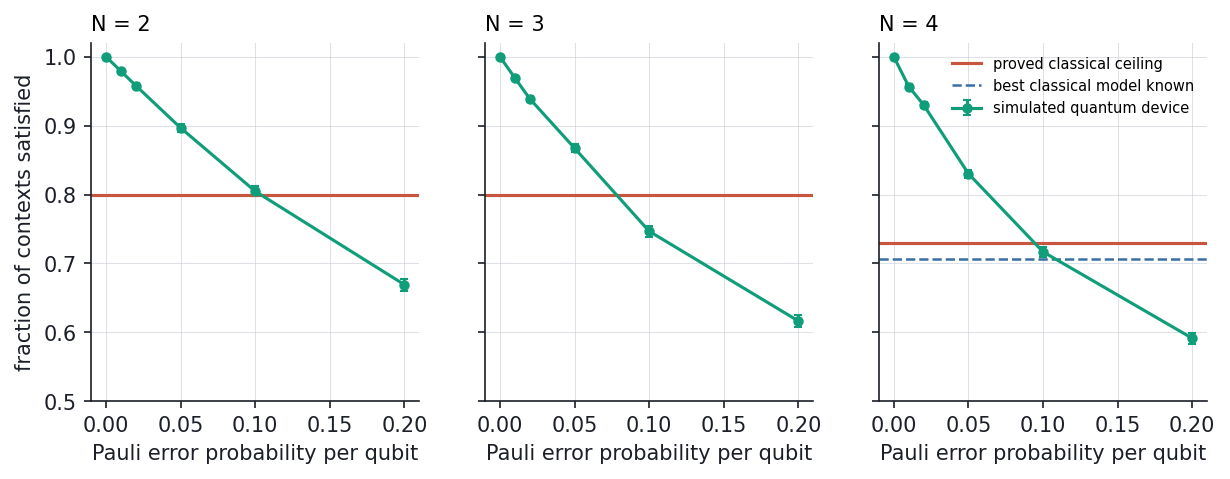
\includegraphics[keepaspectratio,alt={Figure S1}]{figures/fig2_noise.png}}

\emph{Figure S1. Simulated success fraction on Moonlab against the classical ceilings, for the full space.}

\textbf{QGTL} (\texttt{src/qgt\_hoggar.c}, \texttt{src/qgt\_flat.c}). The kernels \texttt{diffgeo\_compute\_fubini\_study} and
\texttt{diffgeo\_compute\_berry\_curvature}, applied to \(\psi_H\) and the 63 tangent vectors \(-\tfrac{i}{2}P_v\psi_H\),
return the values of Proposition 3 to \(10^{-16}\), and the 189 pairs with \(|g_{uv}| \gt 1/12\) are exactly
the pairs on the 63 violated contexts. For the eight states of Table 3 and the tangent vectors of their
supports they return the three values of Proposition 8 to \(10^{-16}\); the pairs above the threshold
recover the 75 violated contexts of \(S_B\) (225 pairs of 9045), the 480 of \(S_5\) and of the support of
\(\Phi_5\) (1440 pairs of 122760), and the 729 344 of \(S_7\) (2 188 032 pairs of 33 028 128), and no others.

\textbf{Eshkol} (\texttt{src/eshkol/hoggar.esk}, \texttt{src/eshkol/saturated.esk}). An exhaustive pass over all \(2^{15}\)
two-qubit assignments gives minimum 3, attained 640 times. The Hoggar signs violate 63 contexts.
Reverse-mode automatic differentiation of the cubic form at the Hoggar Pauli vector \(x^\ast\) gives
\(T(x^\ast) = 7 = (D-1)(D-2)/6\) and \(\nabla T(x^\ast) = 3x^\ast\) to \(7\times10^{-16}\) (the Lagrange condition
for a maximizer on the sphere); nested forward-mode second derivatives along four tangent directions are
negative (\(-0.59\) to \(-0.74\)). For the pivot state the second script finds 135 non-zero expectation
values, 1095 contexts and 75 violated ones, \(T = 35 = (D-1)(D-2)/6\), and \(\nabla T = 7x\) to
\(1.3\times10^{-15}\), which is condition (d) of Theorem 4.

\subsection{S2. Falsifiability and replication}\label{s2-falsifiability-and-replication}

\textbf{Predictions that could fail.} (P1) No assignment violates fewer contexts than the floor. (P2) The
saturated cases are reached exactly. (P3) For every \(S\) and \(f\), \(\operatorname{tr}A = 0\),
\(\operatorname{tr}A^2 = D|S|\), \(\operatorname{tr}A^3 = 6D\beta\). (P4) On an elliptic quadric the spectrum of
\(A\) is doubly degenerate. (P5) For every pure state \(T(p) = (D-1)(D-2)/6\). (P6) Ideal sequential
measurements reproduce every context sign in every state. (P7) For a flat state, condition (d) of
Theorem 4 holds. A single counterexample to P1 would be an assignment whose violation count anyone can
recompute in milliseconds.

\textbf{Tests} (\texttt{scripts/run\_all.sh}).

\begin{itemize}
\tightlist
\item
  \texttt{hoggar\ exhaust2}: all 32768 two-qubit assignments; minimum 3 (640 assignments); for the square,
  minimum 1.
\item
  \texttt{scripts/run\_falsify.sh}: 20 runs over \(N = 2, \dots, 5\) and the three families; 20000, 5000 and 500
  uniformly random assignments and 1500, 200 and 12 annealed ones per configuration for
  \(N = 3, 4, 5\). No assignment below the floor. Minima reached by annealing: 63, 21, 9 (\(N=3\));
  1575, 315, 315 (\(N=4\)); 31479, 6975, 7087 (\(N=5\)). These equal the best known values in every case.
\item
  A negative control: the false claim \(d(W(5,2)) \ge 64\) is refuted by the Hoggar witness with exit
  code 3, showing that the harness can fail.
\item
  \texttt{scripts/flat\_states.py} (68 checks, integer arithmetic in \(\mathbb{Z}[i]\) except one labelled check):
  for the six states of Table 3, the single modulus, the support, the number of contexts, the number
  violated, the floor, condition (d) at every point and the vanishing of every outside sum; the statements
  of Theorem 5 about \(S_B\); Proposition 6 on all 4096 phase patterns; Proposition 9 for one to four
  qubits; and an annealing search from random starts on \(S_B\) and \(S_5\), which reaches 75 and 480 and
  never goes below.
\item
  \texttt{build/third\_level} (seven seconds): the enumeration of Theorem 12, all 33 554 431 forms for five
  qubits included, with the orbit computation; it fails if any count differs from the table.
\item
  \texttt{scripts/phase\_states.py} (81 checks, integer arithmetic): for \(CS|{+}{+}\rangle\), \(CCZ|{+}{+}{+}\rangle\),
  \(CS\,CS|{+}{+}{+}\rangle\), \(\Phi_5\) and \(\Phi_7\), the constant rank, the single modulus, the support, the
  numbers of contexts and violated contexts, condition (d) and the outside sums, and the description of
  the support in Proposition 11; Proposition 10 for all eleven states of this paper; the enumeration of
  Theorem 12 for \(N \le 4\) by a second implementation; the two symplectic maps of Theorem 12; and the
  finite-field descriptions of the five- and seven-qubit forms.
\item
  \texttt{scripts/run\_family7.sh} (about eight core-hours, not part of the everyday run): the enumeration of
  Theorem 13, the orbit computation, and the random census of the other types; its output is
  \texttt{results/family7.log}. The two counts agree: 13 271 040 solutions found, and
  \(92\,897\,280/7 = 13\,271\,040\) for one orbit with a stabilizer of order 7.
\item
  The seven-qubit numbers 8128, 2 824 192 and 729 344 are computed three times without shared code: in
  Python with exact integers, in C from the masks (inside the QGTL program) and in JavaScript from the
  expectation values returned by Moonlab.
\item
  \texttt{scripts/analysis.py} (62 checks) and \texttt{scripts/ladder.py} (14 checks): P3 on random data to machine
  precision; P4 on all 120 four-qubit elliptic quadrics; P5; the geometry of the violated sets; closed-form
  counts against enumeration; agreement of the C and Python integer bounds.
\item
  Witness files (\texttt{data/witness/}, \texttt{data/flat/}) are recounted by independent routines that use no tables.
\end{itemize}

\textbf{Independent implementations.} The geometry, the context signs and the counts are implemented five
times: C (\texttt{src/hoggar.c}), Python with explicit matrices or exact integers (\texttt{scripts/analysis.py},
\texttt{scripts/flat\_states.py}), JavaScript (\texttt{src/moonlab\_experiment.mjs}, \texttt{src/moonlab\_saturated.mjs}),
Eshkol, and the Lean model, in which the signs are theorems about matrix products. They agree on every
number in this paper.

\subsection{S3. Reproduction}\label{s3-reproduction}

\begin{verbatim}
# engine, random source, QGT programs (gcc; no other dependency)
bash scripts/build.sh
# every test: exhaustive N=2, falsification suite, flat states, analysis, ladder, Moonlab, QGTL, Eshkol
bash scripts/run_all.sh
# Lean (needs elan; fetches Lean 4.35.0 and the Mathlib cache)
cd lean && lake exe cache get && lake build
# the exact degrees of Section 5 (kernel evaluations; about a quarter of an hour, under 5 GB each)
lake build HoggarBound.Saturated HoggarBound.SaturatedPhaseFive
lake env lean SaturatedVerification.lean
# the seven-qubit enumeration of Theorem 13 (about eight core-hours)
cd .. && bash scripts/run_family7.sh
\end{verbatim}

\subsection{S4. Witness assignments}\label{s4-witness-assignments}

\texttt{data/witness/nN\_t.txt} holds, for \(N\) qubits and family \(t\) (\texttt{f} full, \texttt{h} hyperbolic, \texttt{e} elliptic), one
header line and a hexadecimal mask whose bit \(v\) is set when \(f(v) = -1\), with \(v = a + 2^N c\). The
three-qubit Hoggar witness produced by the Moonlab run is

\begin{verbatim}
3 f 63
163e5efe76fefe00
\end{verbatim}

\texttt{build/hoggar\ verify\ N\ t\ file} recounts any witness from the definitions.

\texttt{data/flat/nN\_name.txt} holds the configurations of Table 3: a header line with \(N\), the numbers of
observables and contexts and the degree; the mask of the configuration; and the mask of the optimal
assignment. For the pivot configuration:

\begin{verbatim}
4 135 1095 75
b4451eef7889d22344b5ee1f887922d34b45e1ef87892d23bbb5111f7779ddd2
20011cc01888c2204424221f001100c34244212f01010c038880111177790000
\end{verbatim}

The same two numbers are \texttt{pivotMask} and \texttt{pivotNeg} in \texttt{lean/HoggarBound/FlatData.lean}. The files
\texttt{n5\_phase5.txt} and \texttt{n7\_phase7.txt} hold the supports of \(\Phi_5\) and \(\Phi_7\) in the same format; the
seven-qubit masks have 4096 hexadecimal digits.

\end{document}
